\documentclass[12pt, a4paper]{article}
\usepackage{graphicx}
\usepackage{amsmath}


\begin{document}
\title{Sea-ice Flow Simplified}
\author{Kecheng Zhang}
\maketitle

\begin{abstract}
    
\end{abstract}

\section{Introduction}
This is an Introduction

\section{Method}

\subsection{Mathematics}
The speed of the piece can be modeled as
$$ U = 0.5 + 0.3sin(2 \pi x) $$
where x is the position of the piece, and we have data
$x_1(0) = 0.3$, $x_2(0) = 0.7$, and $v_1(0) = v_2(0) = 0$.
We want to calculate
$x_k(t_j)$ and $v_k(t_j)$ for $k = 1, 2$ and $j = 1\dots10000$, where
$\delta t = 10^{-3}$ and $t_j = \delta t j$, such that
$$\begin{cases}
    \frac{\partial x_k}{\partial t} = v_k\\
    \frac{\partial v_k}{\partial t} = (u - v_k) |u - v_k|\\
    \end{cases}$$
and $$ \frac{x_k(t_{j+1}) - x_k(t_j)}{dt} = v_k(t_j)$$

\subsection{Neural Network}
The neural network is a feed-forward network with 2 hidden layers shown in Figure 1.

\begin{figure}
    \centering
    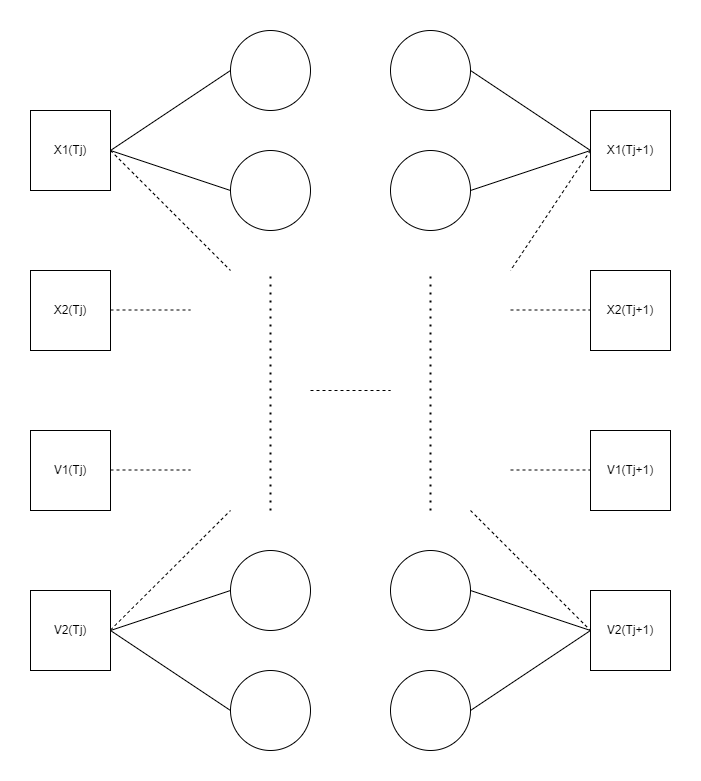
\includegraphics[scale=0.5]{../NN_graph.png}
    \caption[]{Neural Network structure}
    \label{fig:neural_network}
\end{figure}

\section{Discussion}


\end{document}